\documentclass[../D1.tex]{subfiles}

\begin{document}
\subsection{Research questions}
The following are the questions this research will seek to investigate:

\begin{itemize}
    \item Application of pruning algorithms on neural networks: how does changing the pruning paradigm impact latency? (Objectives \hyperref[obj:EvalE2E]{O3}, \hyperref[obj:EvalLayer]{O4}, and \hyperref[obj:EvalComp]{O5})
    \item Can we apply hyperparameter optimisation methods to neural network pruners to minimize latency? (Objective \hyperref[obj:CompPara]{O7})
    \item To what degree can we improve latency (if at all) using an automated strategy while keeping the accuracy metrics above a set threshold? (Objective \hyperref[obj:TestOpt]{O8})
\end{itemize}

\subsection{Research Methodology}
\subsubsection{Core Technology Summary}
This sections provides a brief summary of the core technologies that will be utilised, the core functionality will be written in Python, a combination of different Python versions will be necessary to properly utilise Distiller and OpenVINO.
This versioning issue is one of the reasons we use Redis, it can act as a message broker between Distiller and OpenVINO, we can facilitate a more flexible development by adopting this strategy (inference and training will be completely decoupled).  
\begin{itemize}
    \item \href{https://github.com/IntelLabs/distiller}{Distiller} - A neural network compression library.
    \item \href{https://github.com/openvinotoolkit/openvino}{OpenVINO} - A toolkit to perform inference.
    \item \href{https://github.com/wandb/client}{Weights \& Biases} - A tool for metric recording, visualisation, and parameter optimisation \autocite{biewaldExperimentTrackingWeights}.
    \item \href{https://redis.io/}{Redis} - A fast data structure store (used for FIFO queue).
\end{itemize}


\subsubsection{Compression}
The Distiller library was selected as the platform of choice to perform compression because it functions as a convienent toolbox to test a selection of compression methods under a common environment, and critically a larg collection of compression methods~~\autocite{zmoraNeuralNetworkDistiller2019}.
The decision to use Distiller is reinforced by \hyperref[Aim1]{Aim 1}, there is a rich selection of already-implemented (off-the-shelf) algorithms to choose from, the parameters of these compression algorithms are all defined according to a ``scheduling recipe'' that can be defined programmaatically~\autocite{zmoraNeuralNetworkDistiller2019}.
This project focuses specifically on the pruning methods within distiller, thus we refer to the parts of the scheduling recipe concerned with pruners as the compression parameters, depending on the compression method being used these can be lists of layers to apply the method, initial \& final sparsity, and groupings of the layer structure (channel vs filter).


We will need to consider the schedule for the learning-rate decay class to properly fine tune the model, we will define a fixed learning-rate decay for all experiments to imporove reliability of our results and reduce the search dimensions for our own optimiser.

Fig.~\ref{fig:DistillerArch} Shows a high level view of the Distiller library, to accomplish objective \hyperref[obj:CompPara]{O7} we will primarily be interacting with the scheduler via the interface specified in objective \hyperref[obj:CompPara]{O7}.

\begin{figure}[h]
    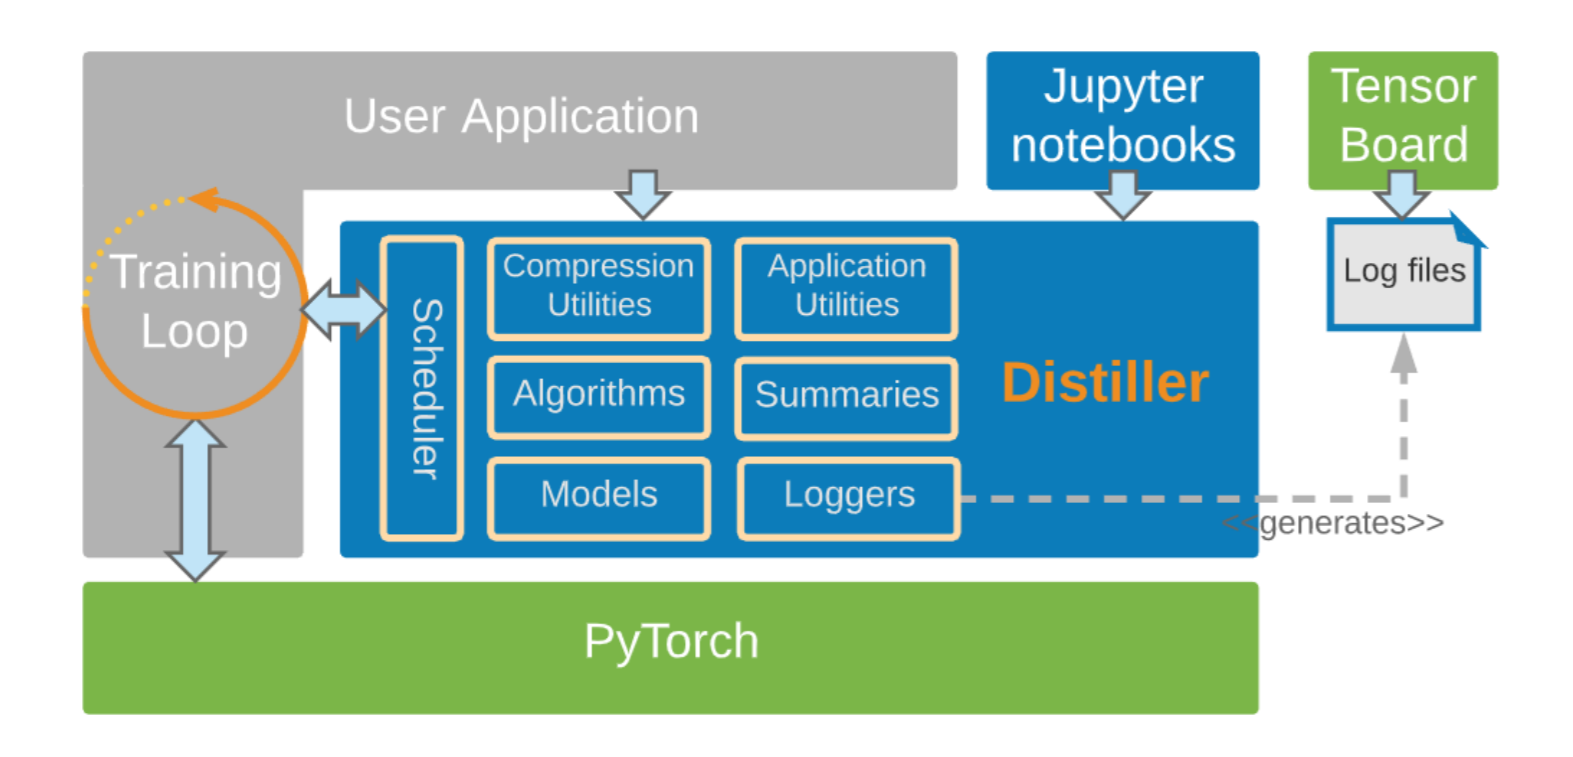
\includegraphics[width=1\textwidth]{DistillerArch.png}
    \caption{Distiller high-level architecture.\\ \textbf{Figure adopted from~\autocite{zmoraNeuralNetworkDistiller2019}}}
    \label{fig:DistillerArch}
\end{figure}

Upon finishing training the Top1 and Top5 metrics will be recorded, ready to be recorded using Weights and Biases with the benchmark metrics when they are ready. 

\subsubsection{Benchmarking}
OpenVINO will be the means by which we perform inference, and evaluate the latency of the compressed models (Objectives \hyperref[obj:EvalE2E]{O3}, \hyperref[obj:EvalLayer]{O4}, and \hyperref[obj:EvalComp]{O5}).
OpenVINO provides a deep learning deployment toolkit via an inference engine, it is compatible with the Neural Compute Stick and has many useful tools to produce metrics related to model and hardware performance.

Benchmarking will be performed using OpenVINO's built in benchmarking tool, we will record inference latency, individual layer latency, and a throughput metric (FPS). 
These metrics can be dumped into an easiliy processable .csv format, we will pass this data back to the training agent once the inference benchmark completes.


\subsubsection{Manual Compression Parameter Selection}
Using the layerwise benchmarking data we will attempt to filter out pruning algorithms that show a detrimental or negative imporvement in latency (\hyperref[Aim1]{Aim 1}), this will reduce the scope of the problem and provide a narrower search space for optimisation (\hyperref[Aim2]{Aim 2}).

\subsubsection{Optimisation}
To automate compression parameter tuning (Objective \hyperref[obj:CompPara]{O7}) we will use a bayesian optimisation technique that models the performance as a sample from a Gaussian process~\autocite{snoekPracticalBayesianOptimization2012}.
Convienently this process is neatly implemented in a machine learning data collection and visualisation tool know as Weights and Biases.



\end{document}